\documentclass[9pt]{beamer}

\usepackage[T1]{fontenc}
\usepackage[utf8]{inputenc}
\usepackage[frenchb]{babel}
\usepackage{eurosym}

\usepackage{multirow}

\usepackage{graphicx}


\newcommand\host{{\it host} }
\newcommand\device{{\it device} }


% --------- BEGIN STYLE BEAMER ---------
\usetheme{Madrid}
\definecolor{ECNBleu}{HTML}{102648}
\definecolor{ECNJaune}{HTML}{FAB600}

\setbeamercolor{frametitle}{bg=ECNBleu,fg=white} %le titre de la frame, en haut
\setbeamercolor{title in head/foot}{bg=ECNJaune,fg=ECNBleu} %barre bas, milieu
\setbeamercolor{author in head/foot}{bg=ECNBleu,fg=ECNJaune} %barre bas, gauche
\setbeamercolor{date in head/foot}{bg=ECNBleu,fg=ECNJaune} %barre bas, droit
\setbeamercolor{section in head/foot}{bg=ECNJaune,fg=ECNBleu} %haut gauche
\setbeamercolor{subsection in head/foot}{bg=ECNBleu,fg=ECNBleu} %haut droite
\setbeamercolor{title}{bg=ECNBleu,fg=white}
\setbeamercolor{block title}{fg=white,bg=ECNBleu}

%\setbeamercolor{normal text}{bg=IUTBleuFonce} %texte
\setbeamercolor{item}{bg=ECNBleu}
\setbeamercolor{subitem}{bg=ECNJaune}
\setbeamercolor{description item}{fg=couleurEmph}
\setbeamercolor{section in toc}{fg=ECNBleu}
%\setbeamercolor{subsubitem}{bg=IUTBleuFonce}

%structure (eq emph dans beamer)
\setbeamercolor{emph}{fg=couleurEmph}
% ----------------------------

\usepackage{listings}

\lstdefinestyle{customc}{
  belowcaptionskip=1\baselineskip,
  breaklines=true,
  frame=L,
  xleftmargin=\parindent,
  language=C,
  showstringspaces=false,
  basicstyle=\tiny\ttfamily,
  keywordstyle=\bfseries\color{green!40!black},
  commentstyle=\itshape\color{purple!40!black},
  identifierstyle=\color{blue},
  stringstyle=\color{orange},
}

\lstset{escapechar=@,style=customc}

\newenvironment<>{questionblock}[1]{%
\setbeamercolor{block title}{bg=ECNJaune,fg=ECNBleu}%
\begin{block}#2{#1}}{\end{block}}

\title[GPGPU]{Programmation sur Processeur Graphique}

\subtitle[\ldots]{
---\\Partie 8 : Considérations sur les performances : memory coalescing}
\author[P.-E. Hladik]{Pierre-Emmanuel Hladik\\\tiny pierre-emmanuel.hladik@ec-nantes.fr}
\institute[Centrale Nantes]{}
\date{\today}

\begin{document}

 \frame{\titlepage}
 
%%%%%%%%%%%%%%%%%%%%%
\begin{frame}[plain]
\frametitle{Bande passante de la mémoire globale}

\begin{itemize}
	\item La mémoire globale d'un dispositif CUDA est implémentée avec des DRAM \vspace{.5em}

	\item {\bf La DRAM est lente}\vspace{.5em}

\end{itemize}

      \centering
	\begin{block}{}
	Les bits de données sont stockés dans des cellules DRAM qui sont de petits condensateurs. La quantité de charge électrique fait la différence entre 0 et 1.

Pour lire les données d'une cellule DRAM, le condensateur doit utiliser sa charge électrique pour alimenter une ligne hautement capacitive menant à un capteur et déclencher son mécanisme de détection qui détermine si la quantité de charge présente dans le condensateur est suffisante pour être considérée comme un "1". Ce processus prend 10 nanosecondes dans les puces DRAM modernes. Cela contraste fortement avec le temps de cycle d'horloge inférieur à la nanoseconde des dispositifs informatiques modernes.

	\end{block}  
\end{frame}
%%%%%%%%%%%%%%%%%%%%%
\begin{frame}[plain]
\frametitle{DRAM burst}

\begin{itemize}
	\item Les DRAM modernes utilisent le parallélisme pour augmenter leur taux d'accès aux données

	\item Chaque fois qu'on accède à un emplacement DRAM, on accède à une série d'emplacements consécutifs comprenant l'emplacement demandé et le contenu d'emplacements proches.

	\item Une fois détectées les données de tous ces emplacements consécutifs sont transférées au processeur. Ces emplacements consécutifs auxquels on accède et qui sont délivrés sont appelés des {\bf bursts} (rafales) de DRAM.

\end{itemize}

\end{frame}


%%%%%%%%%%%%%%%%%%%%%

\begin{frame}[plain]
\frametitle{Memory Coalescing}
      \centering
      \begin{block}{}

\begin{center}
	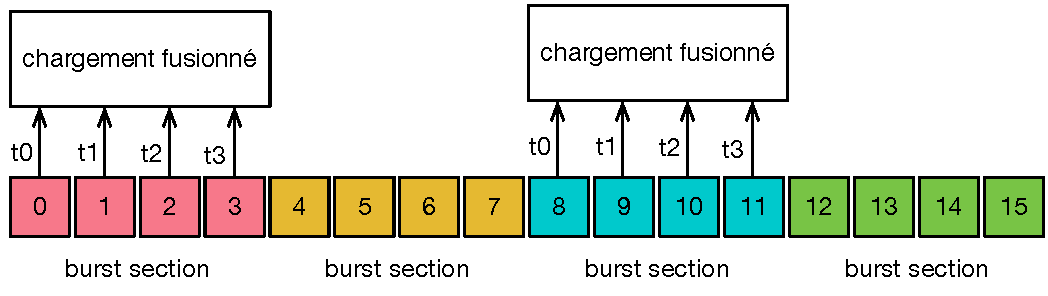
\includegraphics[scale=0.6]{./figures-pdf/coalesced}
\end{center}

Quand les threads exécutent une instruction de chargement, si tous les emplacements accédés tombent dans la même section du brust, une seule demande de DRAM sera faite et l'accès est entièrement fusionné ({\it coalesced})

	\end{block}  
\end{frame}
%%%%%%%%%%%%%%%%%%%%%%%%%%
\begin{frame}[plain]
\frametitle{Accès Un-coalesced}
      \centering
      \begin{block}{}

\begin{center}
	
\includegraphics[scale=0.6]{./figures-pdf/uncoalesced}
\end{center}

Lorsque les adresses accédées par les threads sont sur plusieurs sections de bursts :
\begin{itemize}
\item La fusion échoue
\item Plusieurs demandes de DRAM sont faites
\item Certains des octets auxquels on accède et qui sont transférés ne sont pas utilisés par les threads
\end{itemize}
	\end{block}  
\end{frame}

%%%%%%%%%%%%%%%%%%%%%%%%%%
\begin{frame}[plain,fragile]
\frametitle{Exemple avec la multiplication matricielle naïve}
\begin{lstlisting}[language=C]
__global__
void MatrixMulKernel(float* M, float* N, float* P, int width)
{
  int row = blockIdx.y * blockDim.y + threadIdx.y;
  int col = blockIdx.x * blockDim.x + threadIdx.x;

  if ((row < width) && (col < width)) {
    float sum = 0;
    for (int k = 0; k < width; k++)
    {
      sum += M[row * width + k]*N[k * width + col];
    }
    P[row * width + col] = sum;
  }
 
}
 \end{lstlisting}

\end{frame}
%%%%%%%%%%%%%%%%%%%%%%%%%%
\begin{frame}[plain,fragile]
\frametitle{Exemple : produit matriciel -- accès fusionné}
\begin{center}
	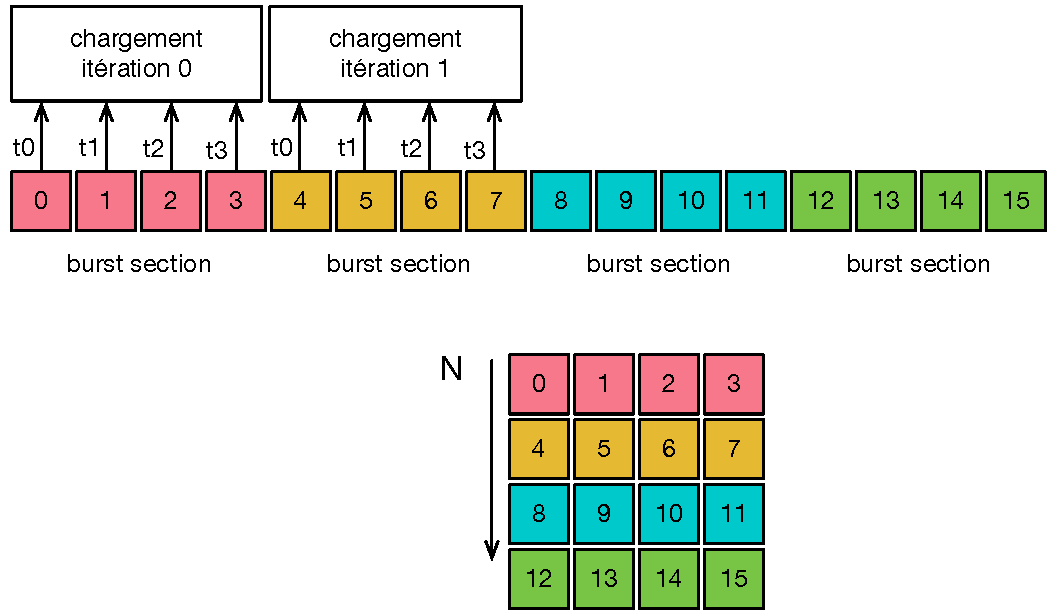
\includegraphics[scale=0.5]{./figures-pdf/N_coalescend}
\end{center}
\end{frame}
%%%%%%%%%%%%%%%%%%%%%%%%%%
\begin{frame}[plain,fragile]
\frametitle{Exemple : produit matriciel -- accès non fusionné}
\begin{center}
	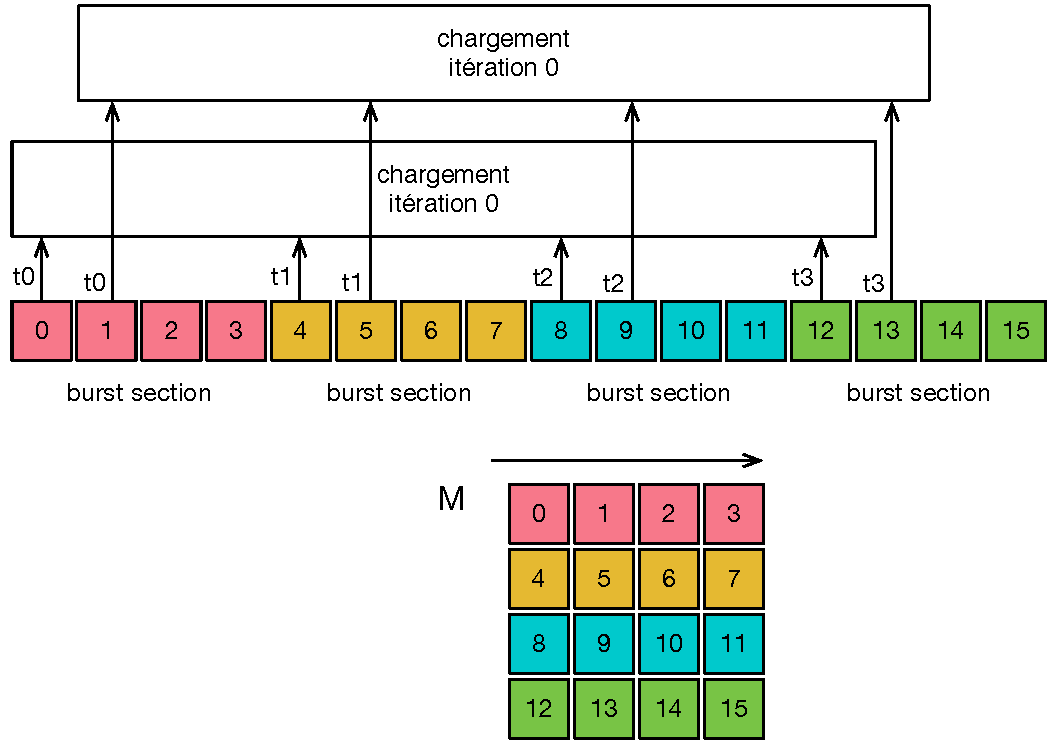
\includegraphics[scale=0.5]{./figures-pdf/M_uncoalescend}
\end{center}


\end{frame}
%%%%%%%%%%%%%%%%%%%%%%%%%%

%%%%%%%%%%%%%%%%%%%%%%%%%%
\begin{frame}[plain,fragile]
\frametitle{Caractéristique mémoire de la Jetson Nano}

Caractéristique : 2GB 64-bit LPDDR4; 25.6 gigabytes/second, soit :
\begin{itemize}
	\item 2Go de mémoire LPDDR4 (Low Power Double Data Rate 4), une mémoire vive à faible consommation énergétique optimisée pour les systèmes embarqués.
	\item un bus mémoire de 64 bits de large, ce qui signifie que chaque accès peut transférer 64 bits (8 octets) à la fois.
	\item avec une bande passante mémoire maximale à 25.6 Go/seconde, qui représente la vitesse théorique à laquelle le système peut lire ou écrire des données en RAM
\end{itemize}

\begin{block}{Taille du "burst"}
Dans les mémoires LPDDR4, un accès en burst signifie que plusieurs mots de données sont lus ou écrits en rafale. La taille minimale d'un burst pour LPDDR4 est généralement 16 mots de 32 bits (soit 64 octets).
\end{block}
\end{frame}
%%%%%%%%%%%%%%%%%%%%%%%%%%
\begin{frame}[plain,fragile]
\frametitle{Exemple avec la multiplication matricielle par tuile }
\begin{lstlisting}[language=C]

__global__
void MatrixMulKernel(float* M, float* N, float* P, int size)
{
  __shared__ float ds_M[TILE_SIZE][TILE_SIZE];
  __shared__ float ds_N[TILE_SIZE][TILE_SIZE];
  
  int bx = blockIdx.x; int by  = blockIdx.y;
  int tx = threadIdx.x; int ty = threadIdx.y;
  int Row = by * blockDim.y + ty;
  int Col = bx * blockDim.x + tx;
  float sum= 0.0;

  for (int p = 0; p < n/TILE_SIZE; ++p) {
    ds_M[ty][tx] = M[Row * size + p * TILE_SIZE + tx];
    ds_N[ty][tx] = N[(p * TILE_SIZE + ty) * size + Col];
    // eq.: ds_N[ty][tx] = N[(p * TILE_SIZE + ty) * size + bx * blockDim.x + tx];
    __syncthreads();
    
    for (int k = 0; k < TILE_SIZE; k++) {
      sum += ds_M[ty][k] * ds_N[k][tx];
    }
    __syncthreads();
  }
  P[Row*size+Col] = sum;
}
 \end{lstlisting}

\end{frame}
%%%%%%%%%%%%%%%%%%%%%%%%%%
\begin{frame}[plain]
\frametitle{Exemple : produit matriciel -- accès fusionné -- warp}
\begin{center}
	\includegraphics[scale=0.7]{./figures-pdf/matrix2}
\end{center}
\end{frame}

%%%%%%%%%%%%%%%%%%%%%%%%%%
\begin{frame}[plain]
\frametitle{Un peu de pratique avec le TD 8}

\begin{block}{Objectifs}
\begin{itemize}
	\item Observer les effets d’un accès fusionnée ou non
\end{itemize}
\end{block}
\end{frame}
%%%%%%%%%%%%%%%%%%%%%%%%%%


%%%%%%%%%%%%%%%%%%%%%%%%%%
\end{document}